\documentclass[12pt,a4paper]{article}
\usepackage{amsmath}
\usepackage{amsfonts}
\usepackage{amssymb}
\usepackage{setspace}
\usepackage{listings}
\usepackage{graphicx}
\usepackage{indentfirst}
\usepackage[normalem]{ulem}
\usepackage[T2A]{fontenc}
\usepackage[utf8]{inputenc}
\usepackage[english,russian]{babel}
%-------------------------------------------
\setlength{\textwidth}{7.0in}
\setlength{\oddsidemargin}{-0.35in}
\setlength{\topmargin}{-0.5in}
\setlength{\textheight}{9.0in}
\setlength{\parindent}{0.3in}
\graphicspath{{../plot/}}


\onehalfspacing


\begin{document}

\begin{titlepage}
  \begin{center}
    МИНОБРНАУКИ РОССИИ\\
    САНКТ-ПЕТЕРБУРГСКИЙ ГОСУДАРСТВЕННЫЙ\\
    ЭЛЕКТРОТЕХНИЧЕСКИЙ УНИВЕРСИТЕТ\\
    <<ЛЭТИ>> ИМ. В. И. ЛЕНИНА (УЛЬЯНОВА)\\
    Кафедра МО ЭВМ

    \vspace{4cm}

    ОТЧЕТ\\
    по практической работе №2\\
    по дисциплине <<Теория принятия решений>>\\
    Тема: Бесконечные антагонистические игры
    \vfill

    \begin{tabular}{ c c c }
      Студент гр. 8303 & \uline{\hspace{3cm}} & Гришин К. И. \\[1cm]
      Преподаватель    & \uline{\hspace{3cm}} & Попова Е. В. \\
    \end{tabular}
    
    \vfill
    Санкт-Петербург\\
    2022
  \end{center}
\end{titlepage}


\section{Цель работы}
Использование инструментальных средств для решения задач поддержки
принятия решения, а также овладение навыками принятия решения на основе
бесконечных антагонистических игр.

\section{Основные теоретические положения}
В данной работе рассматриваются антагонистические игры, которые
отличаются от матричных тем, что в них один или оба игрока имеют
бесконечное (счётное или континуум) множество стратегий.
С теоретико-игровой точки зрения это отличие малосущественно, поскольку игра
остаётся антагонистической и проблема состоит в использовании более
сложного аналитического аппарата исследования.

Таким образом, исследуются общие антагонистические игры, т.е. системы
вида:
\[
  \Gamma = (X, Y, H)
\]
где $X$ и $Y$ – произвольные бесконечные множества, элементы которых
являются стратегиями игроков 1 и 2 соответственно,
а $H:X \times Y \rightarrow R^1$ --- функция выигрыша игрока 1.
Выигрыш игрока 2 в ситуации $(x, y)$ равен $[-H(x,y)], x \in X, y \in Y$ (игра антагонистическая).
Далее рассматриваются такие игры, у которых функция $H$ ограничена.

\vspace{.5cm}
Одновременная игра преследования на плоскости

Пусть $S_1$ и $S_2$ – множества на плоскости. Игра $\Gamma$ заключается в следующем.
Игрок 1 выбирает некоторую точку $x \in S_1$ , а игрок 2 выбирает точку $y \in S_2$.
При совершении выбора игроки 1 и 2 не имеют информации о действияхпротивника,
поэтому подобный выбор удобно интерпретировать как одновременный.
В этом случае точки $x \in S_1, y \in S_2$ являются стратегиями игроков
1 и 2 соответственно. Таким образом, множества стратегий игроков совпадают с
множествами и на плоскости.

Целью игрока 2 является минимизация расстояния между ним и игроком 1
(игрок 1 преследует противоположную цель). Поэтому под выигрышем $H(x,y)$
игрока 1 в этой игре понимается евклидово расстояние $\rho(x,y)$ между точками
$x \in S_1$ и $y \in S_2$, т.е. $H(x, y) = \rho(x, y), x \in S_1, y \in S_2$.
Выигрыш игрока 2 полагаем равным выигрышу игрока 1, взятому с обратным знаком,
а именно $[-\rho(x,y)]$ (игра антагонистическая).

\vspace{.5cm}
Модель покера с одним кругом ставок и одним размером ставки.

В начале партии каждый из двух игроков $A$ и $B$ ставит по единице.
После того, как каждый из игроков получит карту, ходит игрок $A$:
он может или поставить ещё $c$ единиц или спасовать и потерять свою начальную ставку.
Если $A$ ставит, то у $B$ две альтернативы: он может или спасовать (теряя при этом
свою начальную ставку), или уровнять, поставив $c$ единиц. Если $B$ уравнивает,
то игроки открывают свои карты и игрок с лучшей картой выигрывает единицу
(банк).

Обозначим карту игрока $A$ через $x$, а карту игрока $B$ через $y$,
при этом предполагаем, что случайные величины $x$ и $y$ имеют
равномерное распределение на единичном интервале.

Стратегии строятся следующим образом. Пусть:
\begin{itemize}
  \item $\alpha(x)$ --- вероятность того, что если $A$ получит $x$, то он поставит $c$
  \item $1 - \alpha(x)$ --- вероятность того, что если $A$ получит $x$, то он спасует
  \item $\beta(y)$ --- вероятность того, что если $B$ получит $x$, то он уровняет ставку $c$
  \item $1 - \beta(y)$ --- вероятность того, что если $A$ получит $x$, то он спасует
\end{itemize}

Если игроки применяют эти стратегии, то ожидаемый чистый выигрыш $K(\alpha, \beta)$
представляет собой сумму выигрышей, соответствующих трём взаимно исключающим
возможностям: $A$ пасует; $A$ ставит $a$ единиц и B уравнивает; $A$ ставит и $B$ пасует.

Для решения игры необходимо найти такую пару стратегий $(\alpha^*, \beta^*)$
которая удовлетворяет для всех стратегий $\alpha$ и $\beta$ соответственно.
$$ K(\alpha, \beta^*) \leq K(\alpha^*, \beta^*) \leq K(\alpha^*, \beta)$$

\section{Задание}
Решить задачи преследования и покера

Вариант 3

\vspace{.5cm}
Для игры преследования:\\
Фигура $S_1$ -- квадрат со стороной $a$\\
Фиугра $S_2$ -- равнобедренный треугольник с основанием $b$ и высотой $h$

\vspace{.5cm}
Для покера:\\
Размер ставки $c = 4$

\pagebreak
\section{Выполнение работы}
\subsection{Игра преследования на плоскости}

Фигуры соосны и отображены на рисунке 1.
\begin{figure}[ht]
  \centering
  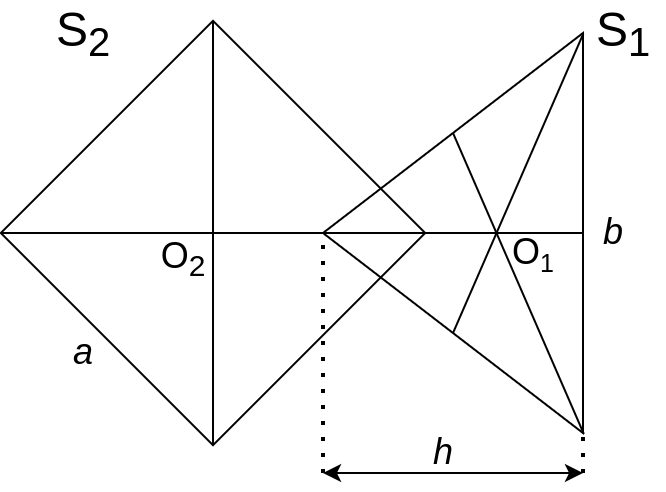
\includegraphics[scale=0.4]{persuit.drawio.png}
  \caption{Представление фигур для случая $O_1 \notin S_2 $}
\end{figure}

Поиск нижней цены игры
Для любой точки $x \in S_1$ и $x \notin S_2$ минимальное расстояние до $S_2$
равно перпендикуляру, опущенному на сторону квадрата $S_2$ (рис. 2).
\begin{figure}[ht]
  \centering
  
\includegraphics[scale=0.4]{persuit_min.drawio.png}
  \caption{Минимальное расстояние от треугольника до квадрата}
\end{figure}

\pagebreak

Из возможных минимальных расстояний, масимальным является то, в которой $x \in S_1$
приходится на одну из вершин, смежных с основанием $S_1$ (рис. 3).
\begin{figure}[ht]
  \centering
  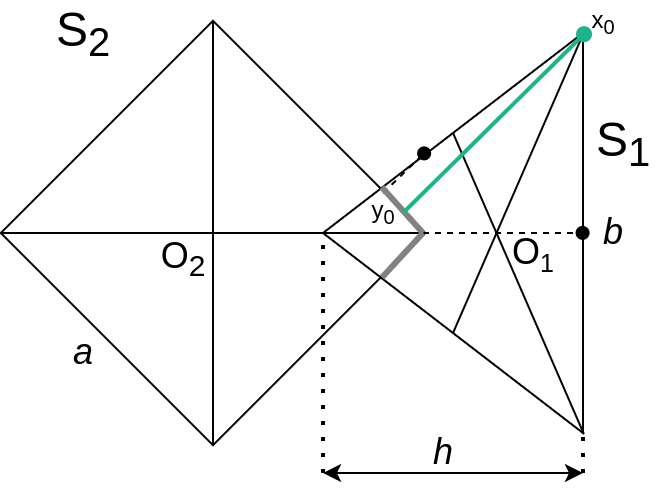
\includegraphics[scale=0.4]{persuit_min_max.drawio.png}
  \caption{Нижняя цена игры}
\end{figure}

Найдем полученное расстояние. Положение точки $x_0$, начало координат в точке $O_2$:
\[
  x_0 = (\|O_1 O_2\|+\frac{bh}{b+\sqrt{4h^2+b^2}}, b/2)
\]

Расстояние от точки $x_0$ до прямой стороны квадрата $S_2$ ($x + y - a/\sqrt{2}=0$):
\[
  \left\vert
    \frac {
      \Vert O_1 O_2 \Vert +
      \dfrac{bh}{b+\sqrt{4h^2+b^2}} +
      \dfrac{b}{2} -
      \sqrt{2}a
    } {
      \sqrt{2}
    }
  \right\vert
\]

Нижняя цена игры:
\[
  \underline{v} = \rho(x_0, y_0) =
  \left\vert
    \frac {
      \Vert O_1 O_2 \Vert +
      \dfrac{bh}{b+\sqrt{4h^2+b^2}} +
      \dfrac{b}{2} -
      \sqrt{2}a
    } {
      \sqrt{2}
    }
  \right\vert
\]

В случае, когда перпидикуляр из вершины треуглоьника $S_1$ не может быть
опущен на сторону квадрата $S_2$:
\[
  h >= b/2, \quad \| O_1 O_2 \| > a + b/2
\]

Максимальным будет расстояние от правого угла квадрата $S_2$,
к точке пересечения перпендикуляра стороны квадрата $S_2$ от этого угла
к стороне треугольника $S_1$ (рис. 4)

\begin{figure}[ht]
  \centering
  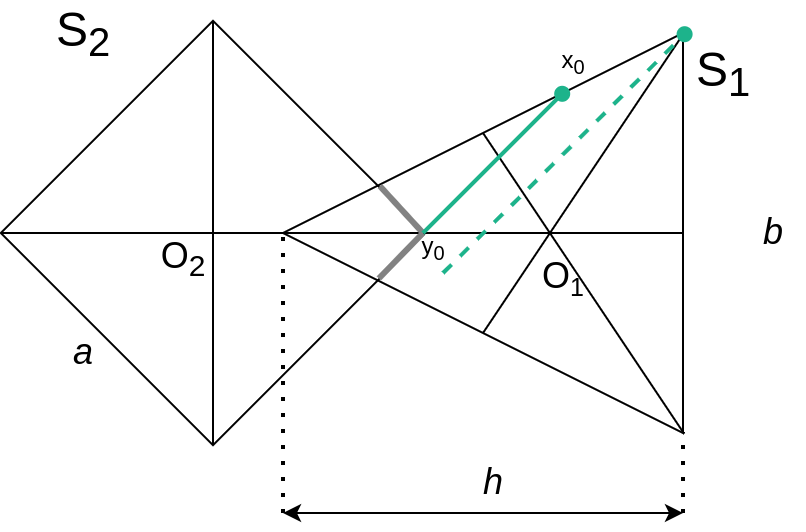
\includegraphics[scale=0.4]{persuit_min_max_3.drawio.png}
  \caption{Нижняя цена игры, при $h >= b/2$, $\| O_1 O_2 \| > a + b/2$}
\end{figure}

Функция стороны квадрата $S_2$:
\[
  x - y - \frac{\sqrt{2}}{2}a = 0
\]

Функция стороны треугольника $S_1$:
\[
  \frac{b}{2h}x - y + \frac{b(h - \|O_1 O_2\|-r)}{2h} = 0, \quad r = \frac{bh}{b+\sqrt{4h^2+b^2}}
\]

Введем обозначения:
\[
  \begin{aligned}
    D = &
    \begin{vmatrix}
      1 & -1 \\
      \dfrac{b}{2h} & - 1
    \end{vmatrix} \\ \vspace{.5cm} \\
    D_x = &
    \begin{vmatrix}
      \dfrac{\sqrt{2}}{2}a & -1 \\ \vspace{0cm}\\
      -\dfrac{b(h - \|O_1 O_2\|-r)}{2h} & - 1
    \end{vmatrix} \\ \vspace{.5cm} \\
    D_y = &
    \begin{vmatrix}
      1 & \dfrac{\sqrt{2}}{2}a \\ \vspace{0cm}\\
      \dfrac{b}{2h} & -\dfrac{b(h - \|O_1 O_2\|-r)}{2h}
    \end{vmatrix}
  \end{aligned}
\]

Тогда нижняя цена игры:
\[
  \underline{v} = \rho(x_0, y_0) =
  \sqrt{\bigl(\frac{D_x}{D} - \frac{\sqrt{2}}{2}a\bigr)^2 + \bigl(\frac{D_y}{D}\bigr)^2} 
\]

В случае, когда $h >= b/2$, $\| O_1 O_2 \| = a + b/2$, нижней ценой игры
является расстояние от правого угла квадрата $S_2$ до смежной с основанием
вершины треуглольника $S_1$

\[
  \underline{v} = \rho(x_0, y_0) = \sqrt{
    \bigl(\frac{\sqrt{2}}{2}a - \|O_1 O_2\|+\frac{bh}{b+\sqrt{4h^2+b^2}}\bigr)^2 +
    \bigl(-\frac{b}{2}\bigr)^2
  }
\]

\vspace{.5cm}
Поиск верхней цены игры.

Для любой точки $y \in S_2$ максимальное расстояние до $S_1$ равно
расстоянию до вершин треугольника $S_1$.
Причем для точек $y$, находящихся в верхней половине квадрата $S_2$, максимальным
будет расстояние до нижней вершины треугольника $S_1$, а для точек $y$ в нижней
половине --- до верхней. Точки, лежащие на горизонтальной диагонали имеют одинаковое
расстояние до любой из вершин (рис. 5).

\begin{figure}[ht]
  \centering
  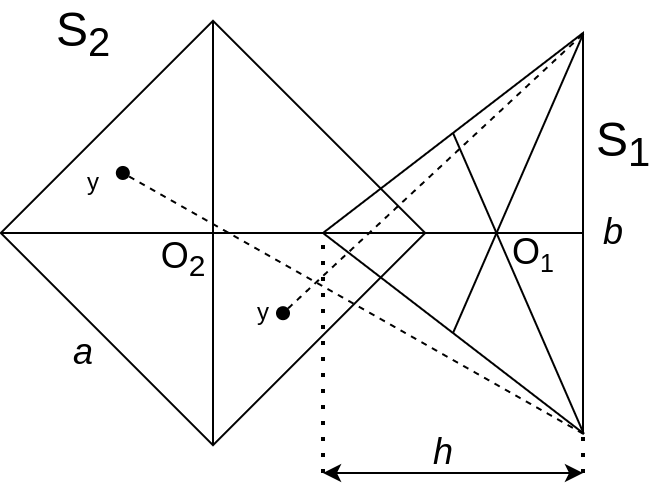
\includegraphics[scale=0.4]{persuit_max.drawio.png}
  \caption{Максимальное расстояние от квадрата до треугольника}
\end{figure}

Из возможных максимальных расстояний, минимальным будет то, что идет от
вершины треуглольника до правого угла квадрата (рис. 6).

\begin{figure}[ht]
  \centering
  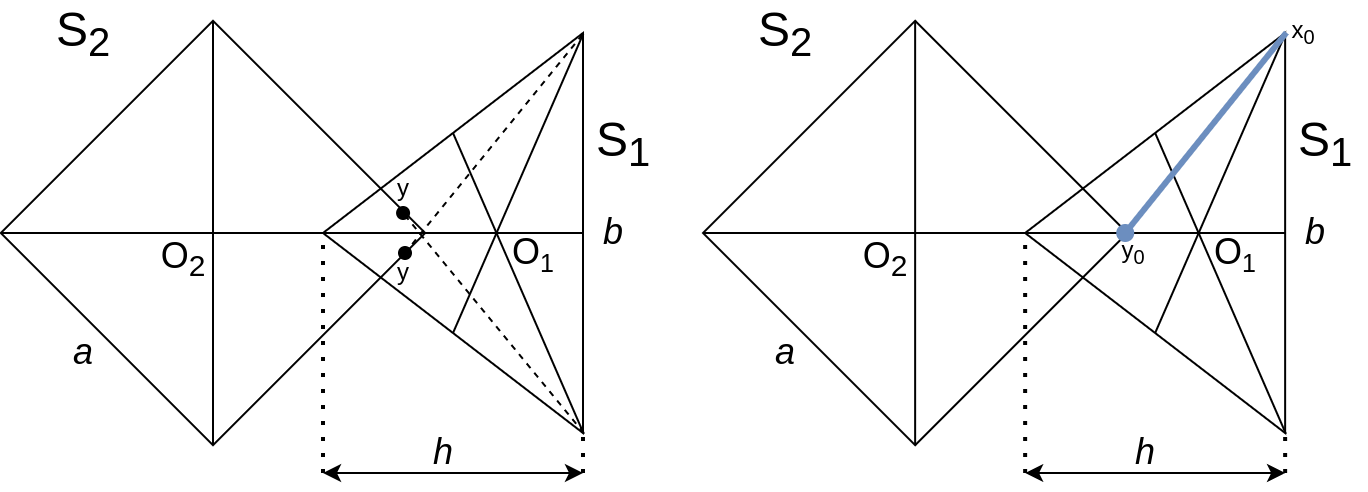
\includegraphics[scale=0.28]{persuit_max_min.drawio.png}
  \caption{Верхняя цена игры}
\end{figure}

Найдем полученное расстояние.\\
Положение точки $x_0$:
\[
  x_0 = (\|O_1 O_2\|+\frac{bh}{b+\sqrt{4h^2+b^2}}, b/2)
\]
Положение точки $y_0$:
\[
  y_0 = (\frac{\sqrt{2}}{2}a, 0)
\]

Расстояние между точками:
\[
  \rho(x_0, y_0) = \sqrt{
    \bigl(\frac{\sqrt{2}}{2}a - \|O_1 O_2\|+\frac{bh}{b+\sqrt{4h^2+b^2}}\bigr)^2 +
    \bigl(-\frac{b}{2}\bigr)^2
  }
\]

Верхняя цена игры:
\[
  \overline{v} = \rho(x_0, y_0) = \sqrt{
    \bigl(\frac{\sqrt{2}}{2}a - \|O_1 O_2\|+\frac{bh}{b+\sqrt{4h^2+b^2}}\bigr)^2 +
    \bigl(-\frac{b}{2}\bigr)^2
  }
\]

\vspace{.5cm}
В случе, когда центр масс $O_1$ принадлежит $S_2$ значения верхней (рис. 7)
и нижней (рис. 8) цены игры не меняются.

\begin{figure}[ht]
  \centering
  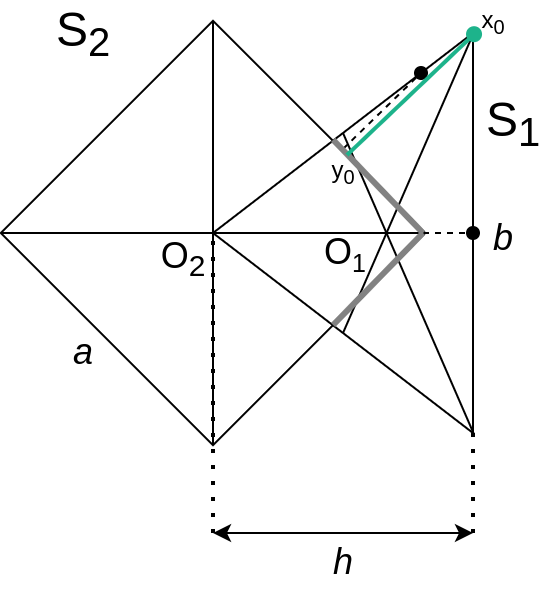
\includegraphics[scale=0.28]{persuit_min_max_2.drawio.png}
  \caption{Нижняя цена игры для случая $O_1 \in S_2$}
\end{figure}

\begin{figure}[ht]
  \centering
  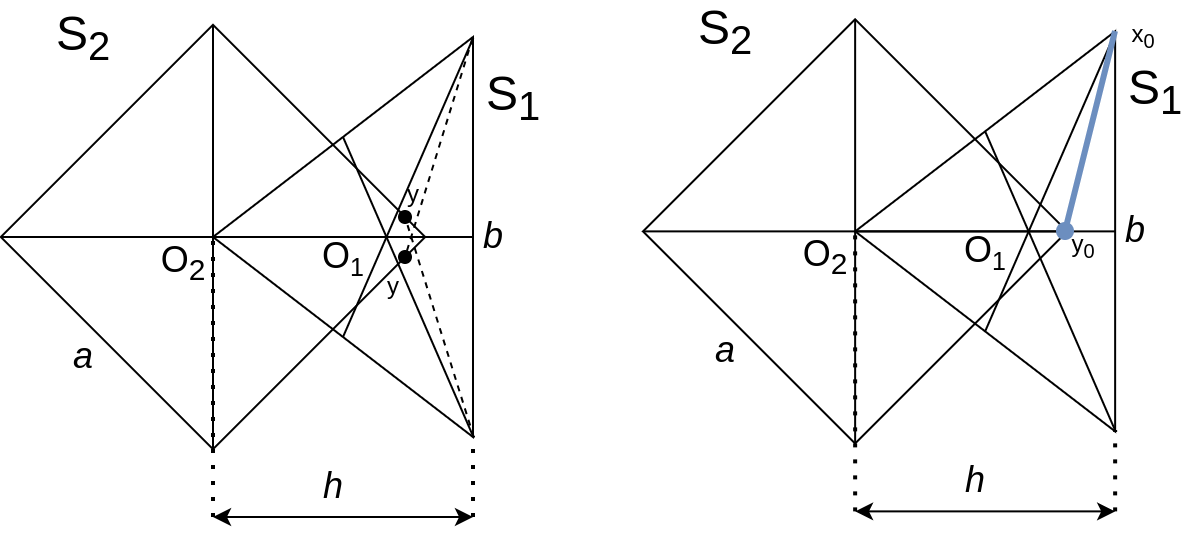
\includegraphics[scale=0.28]{persuit_max_min_2.drawio.png}
  \caption{Верхняя цена игры для случая $O_1 \in S_2$}
\end{figure}


\vspace{.5cm}
\textbf{Ответ:}

В случае когда $O_1 \notin S_2$ и при условии $h >= b/2$, $\| O_1 O_2 \| = a + b/2$
значения верхней и нижней игры совпадают:
\[
  H(x, y) = \underline{v} = \overline{v} = \sqrt{
    \bigl(\frac{\sqrt{2}}{2}a - \|O_1 O_2\|+\frac{bh}{b+\sqrt{4h^2+b^2}}\bigr)^2 +
    \bigl(-\frac{b}{2}\bigr)^2
  }
\]
\pagebreak

\subsection{Задача покера с одним кругом ставок}
Если игрок $A$ использует стратегию $\alpha(x)$ с порогом  $a$, то минимальный
проигрыш $B$ составит:
\[
  H(\alpha,\beta) = \int_{b}^{1} \biggl(-2(c+1)y + a(c+2)+c\biggr) \,dy + 2(1-a)-1
\]

\[
  H(\alpha,\beta) = (c+1)b^2-b(a(c+2)+c)+ac,\:b = \frac{1}{2(c+1)}\bigl(a(c+2)+c\bigr)
\]

\[
  H(\alpha,\beta) = H(a) = \frac{(c+2)^2}{4(c+1)}\bigl(-a^2+2a\frac{c^2}{(c+2)^2} - \frac{c^2}{(c+2)^2}\bigr)
\]

$a$ - стратегия $A$, максимизирующая минимальный проигрыш $B$.

\[
  a = \bigl(\frac{c}{c+2}\bigr)^2, \: a = \frac{4}{9}
\]

$b$ - стратегия $B$, минимизирующая максимальный выигрыш игрока $A$.

\[
  b = \frac{c}{c+2}, \: b = \frac{2}{3}
\]

Подставляя $a$ в $H(a)$, получаем функцию выигрыша от размера ставки $c$.

\[
  \begin{aligned}
    H(\alpha,\beta) = H(a) = H(c) & = \frac{(c+2)^2}{4(c+1)}\bigl(-\bigl(\frac{c}{c+2}\bigr)^4+2\bigl(\frac{c}{c+2}\bigr)^4 - (\frac{c}{(+2})^2\bigr) =\\
    & = \frac{(c+2)^2}{4(c+1)}\bigl(\bigl(\frac{c}{c+2}\bigr)^4 - \frac{c^2}{(c+2)^2}\bigr) = -\frac{c^2}{(c+2)^2}
  \end{aligned}
\]

\begin{center}
  $H(\alpha, \beta) = -\dfrac{4}{9}$, при $c=4$
\end{center}

Игрок $B$ находится в более выигрышном положении, его порог выше, а выигрыш $A$ --- отрицательный.

\vspace{.5cm}
Если
\begin{itemize}
  \item[] $x <   a$, то $\alpha(x) = 0$
  \item[] $x \ge a$, то $\alpha(x) = 1$
  \item[] $y <   b$, то $\beta(y) = 0$
  \item[] $y \ge b$, то $\beta(y) = 1$
\end{itemize}

\pagebreak
Другая стратегия

При использовании оптимальной стратегии $\alpha(x)$ игроком $A$, луший выигрыш
для $B$ получится при использовании стратегии $\beta(y)$ с порогом $b$.

$Q(x)$ для данного $B$:
\[
  \begin{aligned}
    x \leq b \quad & Q(x) = 1 + \int_{0}^{b}dy-\int_{b}^{1}(c+1)dy = 1+b-(c+1)(1-b)=0 \\
    & H(\alpha,\beta)=-1 \\
    x \ge  b \quad & Q(x) = 1 + b \int_{b}^{x}(c+1)dy - \int_{x}^{1}(c+1)dy=2(c+1)x-c(b+1) \ge 0 \\
    & H(\alpha,\beta)=\int_b^1\alpha(x)(2(c+1)x-c(b+1))dx - 1 = \\
    & =2(c+1)\int_b^1xdx-c(b+1)\int_b^1dx-1 = 1 - b^2 -1 = -b^2\\
  \end{aligned}
\]

\[
  H(\alpha,\beta) = -\frac{4}{9}
\]

Если

\begin{itemize}
  \item[] $x \geq b$, игрок $A$ делает ставку;
  \item[] $x \le  b$, игрок $A$ с вероятностью ${p=c/(c+2)=2/3}$ пасует,
  а с вероятностью \\${p=1 - c/(c+2)=1/3}$ --- блефует.
  \item[] $y <   b$, то $\beta(y) = 0$
  \item[] $y \ge b$, то $\beta(y) = 1$
\end{itemize}

\pagebreak

\section{Вывод}
В ходе выполнения практической работы были изучены бесконечные
антагонистические игры, такие как: одновременная игра преследования на
плоскости и покер с одним кругом ставок.

Для одновременной игры преследования на плоскости установлено, что решение
в чистых стратегиях доступно только при соблюдении строгих условий:
\begin{itemize}
  \item Высота треугольника не должна превышать половину основания.
  \item Расстояние между геометрическими центрами должно быть равно сумме
  половины диагонали квадрата и полуоснования.
\end{itemize}

Для игры <<Покер>> с одним кругом ставок было получено, что при
заданном значении ставки выигрыш составит $H(\alpha, \beta) = -4/9$,
что говорит о проигрыше игрока $A$.

\end{document}